\subsection{Anforderungen des Auftraggebers}
Der Auftraggeber teilt seine Anforderungen in notwendige und optionale Ziele ein, welche nachfolgend aufgelistet werden. Die notwendigen Ziele  für den Chatbot sind folgende:

\begin{itemize}
	\item in Slack verwendbar
	\item Datenbank, welche Veranstaltungen und Zuweisungen der Mitglieder enthält
	\item Erfassung, welche Mitglieder wie viele Dienste machen
	\item Abfragefunktion vorhanden
	\item zeitgesteuerte, ereignisbasierte und manuelle Erinnerungsfunktion
	\item Einschränkung der Zielgruppe möglich
	\item einfache Bedienbarkeit
	\item Erweiterbarkeit
	\item MIT-ähnliche Lizenzen für Drittanbietersoftware und -quelltext
	\item Dokumentation der Datenbank
	\item Unabhängkeit der relevanten Daten vom verwendeten Bot
	\item Zukunftssicherheit
\end{itemize}


optionale Ziele
\begin{itemize}
	\item aus iCal Termine extrahieren
	\item Dienstplan aus Doodle-ähnlicher Umfrage erstellen
	\item Nutzerberechtigungen
	\item Steuerung über E-Mail
	\item containerbasierte Lösung
	\item Caching für schnellere Abfragen
	\item Backup-Strategie
\end{itemize}

% Hier schon das Usecase-Diagramm hin? - NEIN, hier kommt nur das rein, was Ferdi gesagt hat. Alles was wir selbst erarbeitet haben kommt danach.

\subsection{Festlegungen}
% Synonyme, Beschreibungen, Abgrenzungen für die Arbeit

Eine Menge an Terminen wird mit $T$ bezeichnet, Veranstaltungen mit $V$ und Sitzungen mit $S$.

\subsection{Anwendungsfalldiagramme}

Die auf den vorherigen Seiten zusammengetragenen obligatorischen Projektziele wurden zur besseren Überprüfung der Ziele in Anwendungsfälle umformuliert. Diese wurden entsprechend \autoref{usecase-auftrag} auf die Akteure \enquote{Bot} und \enquote{Auftraggeber} verteilt.
Der Auftraggeber ist hierbei Hr. Ferdinand Malcher als Vorsitzender des Studentenclubs \enquote{Stecker}, der \enquote{Bot} ist eine nicht näher spezifizierte Chatbot-Technologie, die aber bewusst als Akteur eingeführt wurde, da sie selbständig Aktionen ausführen soll.

\begin{figure}[htbp]
    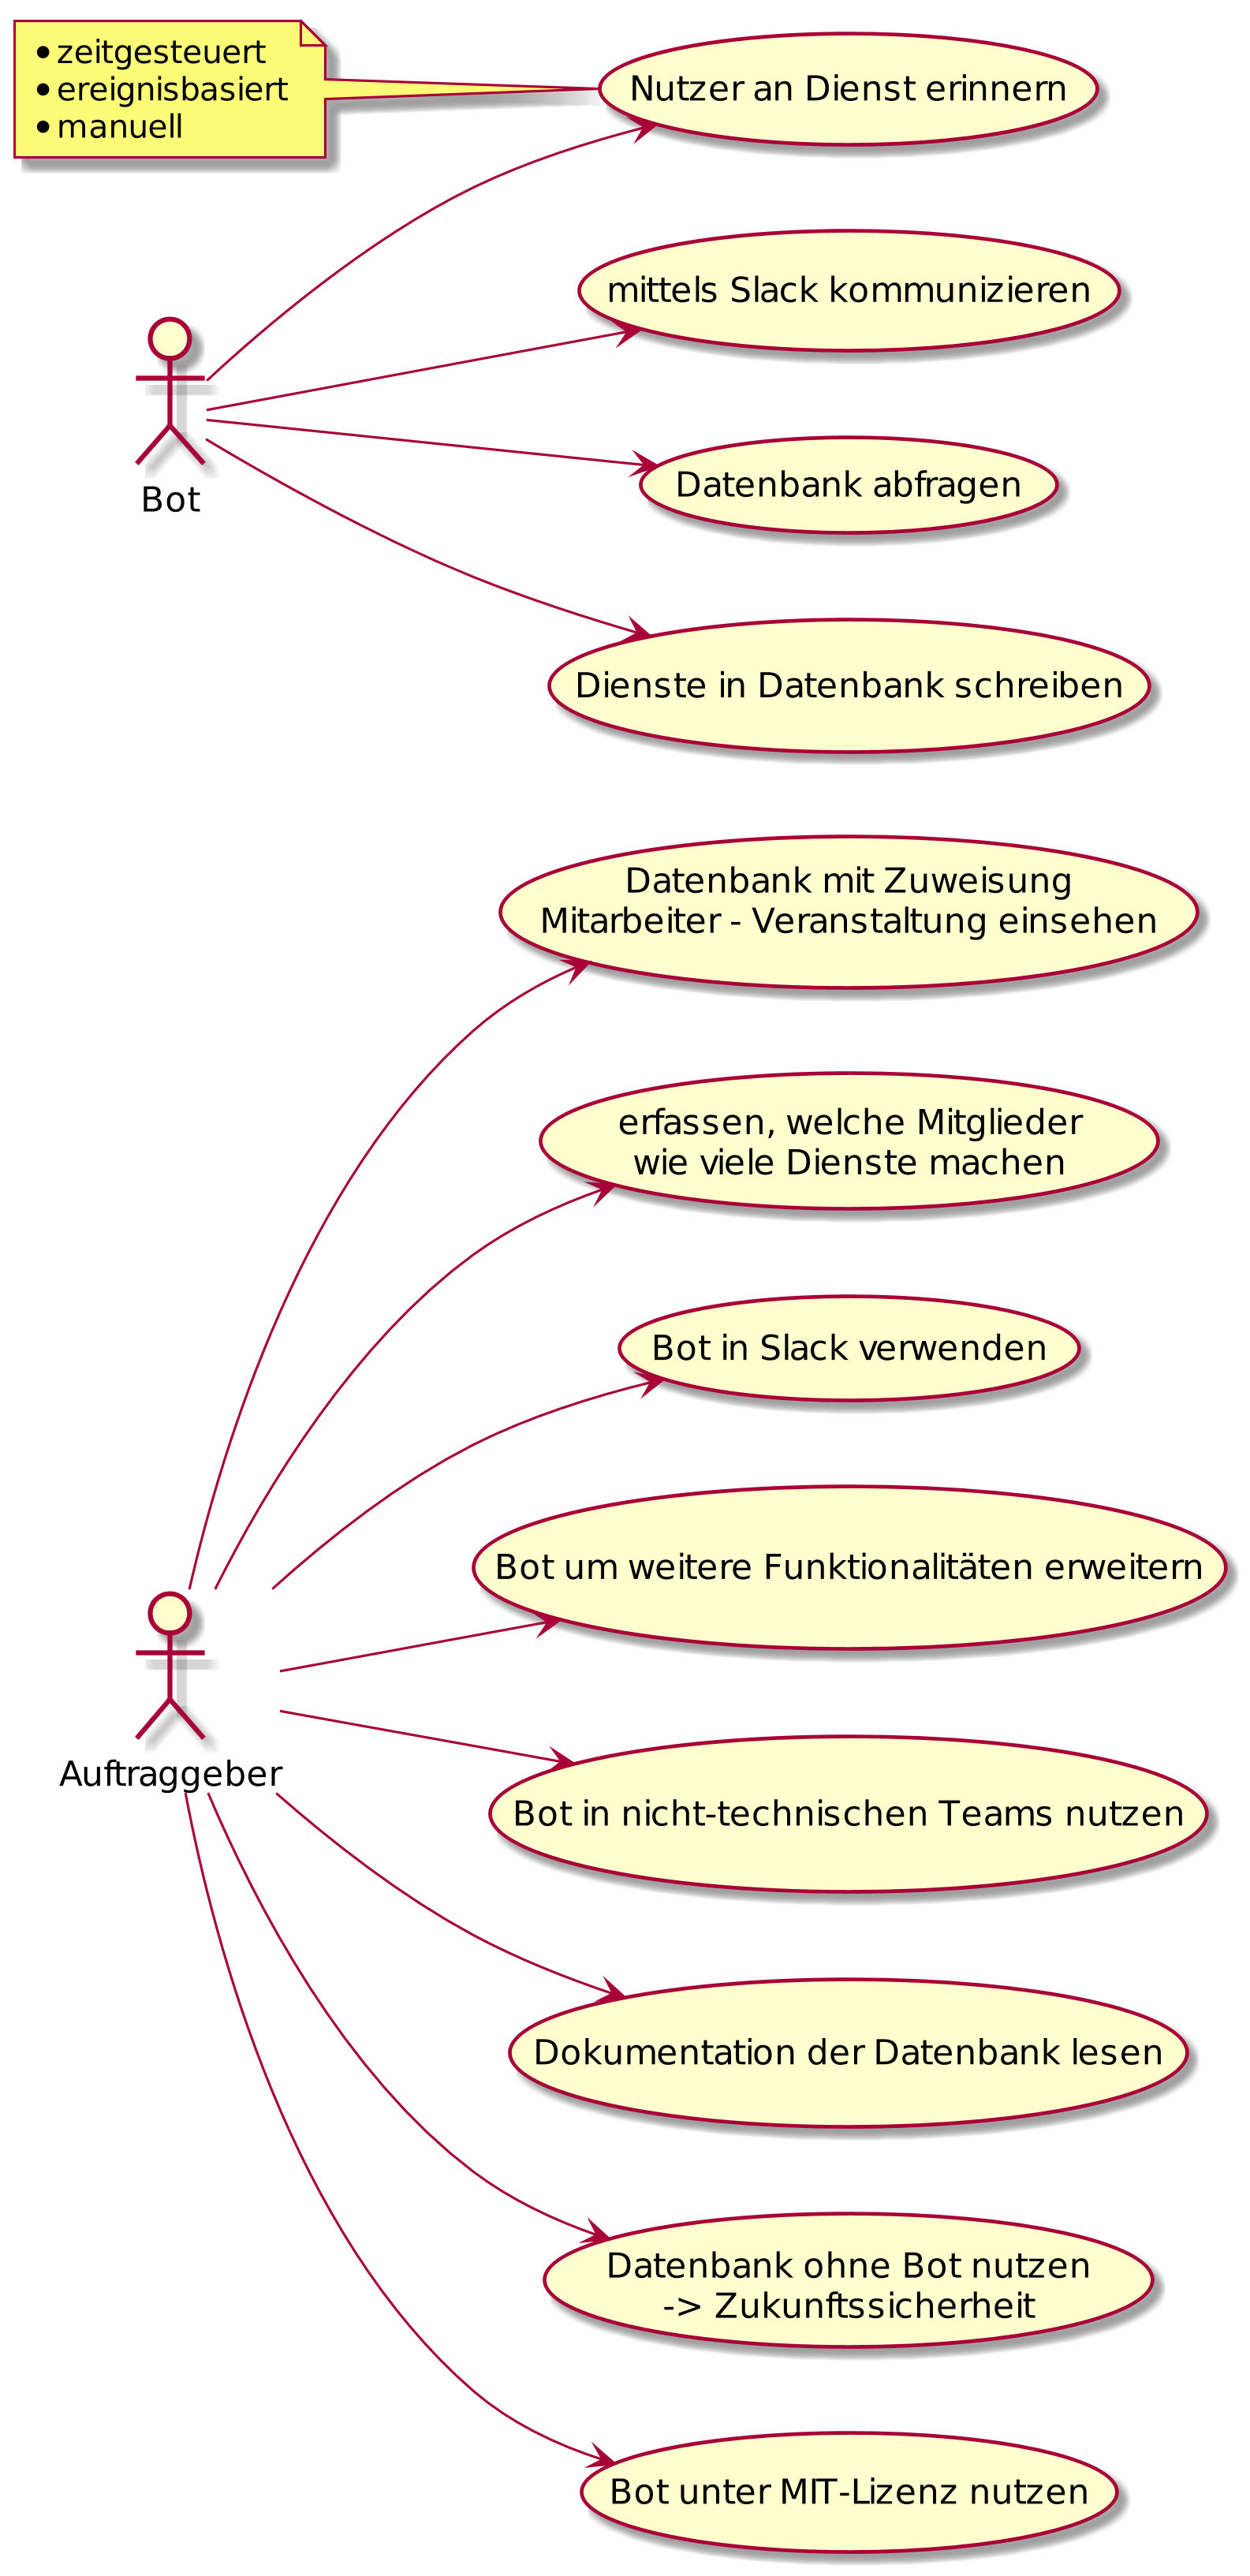
\includegraphics[width=0.7\textwidth]{../docs/uml/usecase-stakeholder.png}
    \caption{Anwendungsfalldiagramm für Auftraggeber und Bot}
    \label{usecase-auftrag}
\end{figure}

